\cleardoublepage
\chapter{The Malleable Document}\label{ch:malleable}  % ``Aims \& objectives''?? Booooring
%The real aim of this project is to produce documents that are adaptable to multiple viewing
%apertures, but do not require total reprocessing to do so.

%Chapter~\ref{ch:intro} goes into considerable detail
%about precisely which elements of a typeset document must be considered
%computation-heavy (and thus should be avoided if possible at view-time).
%This chapter goes some way towards defining exactly which portions of the
%typesetting process can be pre-computed and which cannot. It also analyses where shortcuts
%can be taken, and their effects on the final document.


The invention of movable type in China in the 11th Century, and independently in Europe in the 15th Century, led to an enormous increase in the availability of printed material. Movable type, in various incarnations, formed an enormously important part of the newspaper industry, from its advent in the 17th century until digitisation in the mid-1980s. The inherently volatile nature of newspaper layout (caused, for example, by important stories breaking shortly before going to press) coupled with the expense and time-consuming nature of physical typesetting, led to the development of the familiar columnar appearance of the newspaper that is prevalent worldwide.

\section{The use of Galleys in Typesetting}
In a traditional newspaper layout, each page is divided into columns of equal \emph{measure}, that is of equal horizontal width. All text to appear in the newspaper is typeset to fit this measure (or integer multiples thereof, for example in the case of headlines) allowing articles to be slotted anywhere into the final layout of the newspaper, simply by breaking their text between lines where necessary to span across columns or pages. The article never requires retypesetting as long as its content remains unchanged\ed{}an advantage only available when all text is rendered to the same width.


The metal trays used to contain typeset lines of physical type are known as \emph{galleys}. Newspapers use reasonably narrow galleys; paperback books tend to use wider galleys, and hardback books wider still. \marginpar{A very unscientific survey of various items of print around my desk suggests that newspapers use approximately 2'' galleys, paperback books around 4'', and hardback books around 5''.}Narrower galleys offer the advantage that less space is wasted if the final line in a paragraph does not span the full width: this is more important in newspaper layout than in most other typesetting situations, as space is at a premium. Wider galleys aid readability, up to a certain point, after which it becomes difficult for the eyes to keep track between lines.\cite{Bringhurst2008, Voorhees2011}


Typesetting text into physical galleys is directly analogous to precomputing many of the `hard' parts of typesetting. In particular, all hyphenation, line breaking, justification, kerning, glyph substitution etc. (in fact all horizontal layout) has been `compiled out'. No matter the height of the page nor the number of columns, only vertical layout problems remain, such as attempting to avoid widows and orphans (where the last/first lines of a paragraph appear first/last in a column) and choosing optimal placements of figures and other floating bodies. The problem that remains is similar to that described by Michael Plass in his PhD thesis\cite{Plass1981}.

\section{Galleys as a Reflow Tool}
If an electronic version of a primarily text-based document can be partially pre-rendered into the analogue of a galley, the document is then provided with some limited flowability. Specifically, the document can be rendered for any page size at least as wide as the galley, and of arbitrary height. Wider pages may be able to accommodate multiple columns, but unless the page size is chosen carefully based on the galley's width, there is likely to be noticeable extra horizontal whitespace if the page width is not close to a multiple of the galley width.

\begin{figure}
 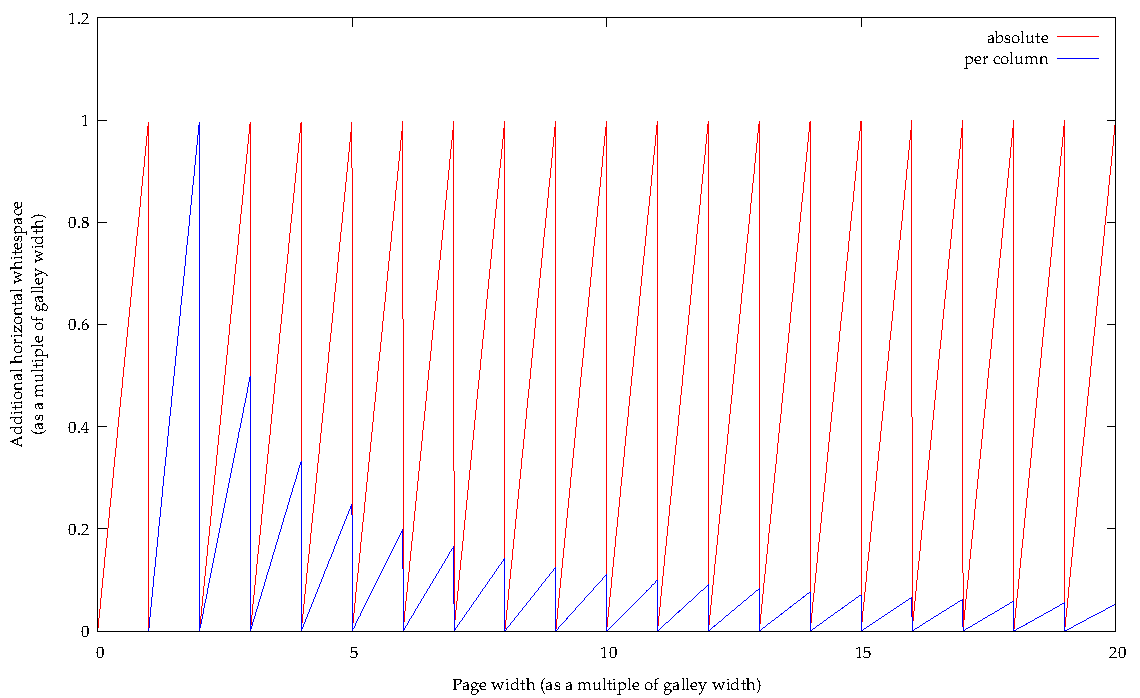
\includegraphics[width=\textwidth]{gnuplot/1col}
 \caption[Extra whitespace in a single-galley document]{As more columns fit on a page, the extra whitespace required per column decreases}
 \label{fig:sawtooth}
\end{figure}


Figure~\ref{fig:sawtooth} shows how the extra horizontal whitespace on a page varies with page width. The peaks are at the point where an extra column can be added, and the amount of extra whitespace required drops to a minimum. The green dashed line divides this extra whitespace by the number of columns on the page, which gives a more useful metric to work with: if we physically divide the extra whitespace and insert it between the columns to increase their spacing (as opposed to leaving it on the right- or left-hand margins) then the wider the page, the less detriment is caused by the extra fraction of galley width.

\section{Multiple Galley Renderings}
The problem of extra whitespace can be overcome in several ways. Firstly, and most simply, the scaling of the galley can be altered, effectively simulating a change in the point size of the font. This is probably undesirable unless a change in point size has explicitly been requested, especially if the size change is particularly noticeable.
A second way in which columns can be better fitted to the page width is to typeset the source document into a range of galleys of varying width. When the document is rendered at view-time, the most appropriate width (according to some metric) can be chosen to be displayed. One very simplistic metric is to choose whichever galley rendering would result in the least extra added whitespace. By overlaying the Figure \mbox{\ref{fig:sawtooth}-like} graphs for each galley, we are able to obtain a graph like Figure~\ref{fig:overlay}, which features all available galleys. If we use our simple metric of minimum whitespace, we can simply choose whichever galley requires the smallest amount of extra whitespace for a given page width.

\begin{figure}
 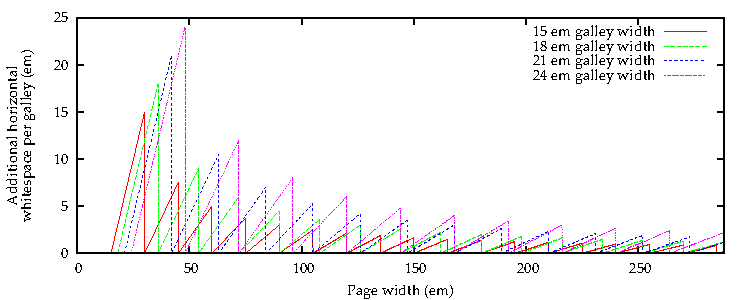
\includegraphics[width=\textwidth]{gnuplot/overlay}
 \caption[Extra whitespace in a multi-galley document]{Overlaying the sawtooth graphs for several galleys of differing widths allows us to minimise the extra added whitespace}
 \label{fig:overlay}
\end{figure}

\section{A Simple Implementation}
At an early stage it was decided that the simplest available method of implementing the above-mentioned layout algorithm was to use some existing tools from the University of Nottingham Document Engineering Laboratory: in particular the Component Object Graphic (\COG{}) model\cite{Bagley2003} for creating and managing modularised \pdf{} documents. This was chosen specifically to avoid the need to write a typesetter or layout engine from scratch; typesetting is performed by the \troff{} suite, and layout by Adobe Acrobat, though there is no reason why this algorithm could not be implemented with any other system capable of tightly specifying page imaging operations. Indeed, for this to be implemented in any non-prototypal form, \ie{} to be used on any portable device, it is likely that a specific, new rendering engine will need to be written for each device (or class of device).

\subsection{The Source Document}\label{sec:srcdoc}
Since the majority of available tools for producing \COG{}ged \pdf{}s rely on the typesetting package \ditroff{}, it was decided to use this as the basis for the source document. \Ditroff{} is particularly amenable to many of the features required here\ed{}it is quite happy to have its page length set to large values\ed{}one sample document used a page length of 2000 inches (approximately 50 metres) with no complaints from \ditroff{}. The line length was set to a small value (approximately two inches) in order to produce a narrow column of text. Following this, the actual document content was inserted several times, incrementing the line length on each iteration, producing one document effectively containing multiple galley-width renderings of the same content.

\subsection{pdfdit}
Having generated the source document, it was processed with ditroff to generate the intermediate code used to feed each typesetter post-pro\-cessor. This output is very expressive, and, unlike \TeX's DVI, contains enough information that post-processors are easily able to locate the start and end of lines and paragraphs within the document. This meant that only minimal changes were needed to be made to the \emph{pdfdit} package described in \cite{Bagley2003} to implement the design.

The first change necessary was to decrease the granularity of the output COGs, producing them at the line level, rather than at the paragraph level. Secondly, some method of generating the requisite tree representing the document structure was required. This was solved by simply using the point at which the original version of pdfdit would have started a new paragraph-level COG, and, instead, starting a new paragraph-level block entry in the document structure tree. Each subsequent line-level COG produced can then be added as a child of this block.

Once the entire output file has been parsed, the tree representations of the various width galleys are amalgamated per-paragraph, as indicated in figure~\ref{fig:tree}, and finally the PDF file is serialised, replete with COGs and content tree.

\begin{figure}
 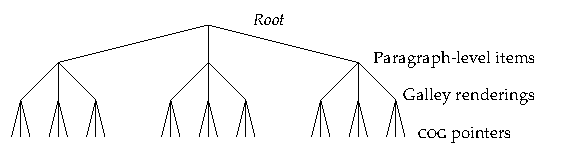
\includegraphics[width=\textwidth]{gfx/tree}
 \caption[A simple document structure tree]{A simple document structure tree. The first level below the root represents all paragraph-level items: headings, paragraphs, figures etc. These items have one child for each galley rendering of the document. These in turn have one child for each \COG{} comprising their content\ed{}in the case of a paragraph or heading its lines; in the case of a figure, the figure itself and any associated caption.}
 \label{fig:tree}
\end{figure}

\subsection{Acrobat Plugin}\label{sec:acroplugin}
\begin{figure}
 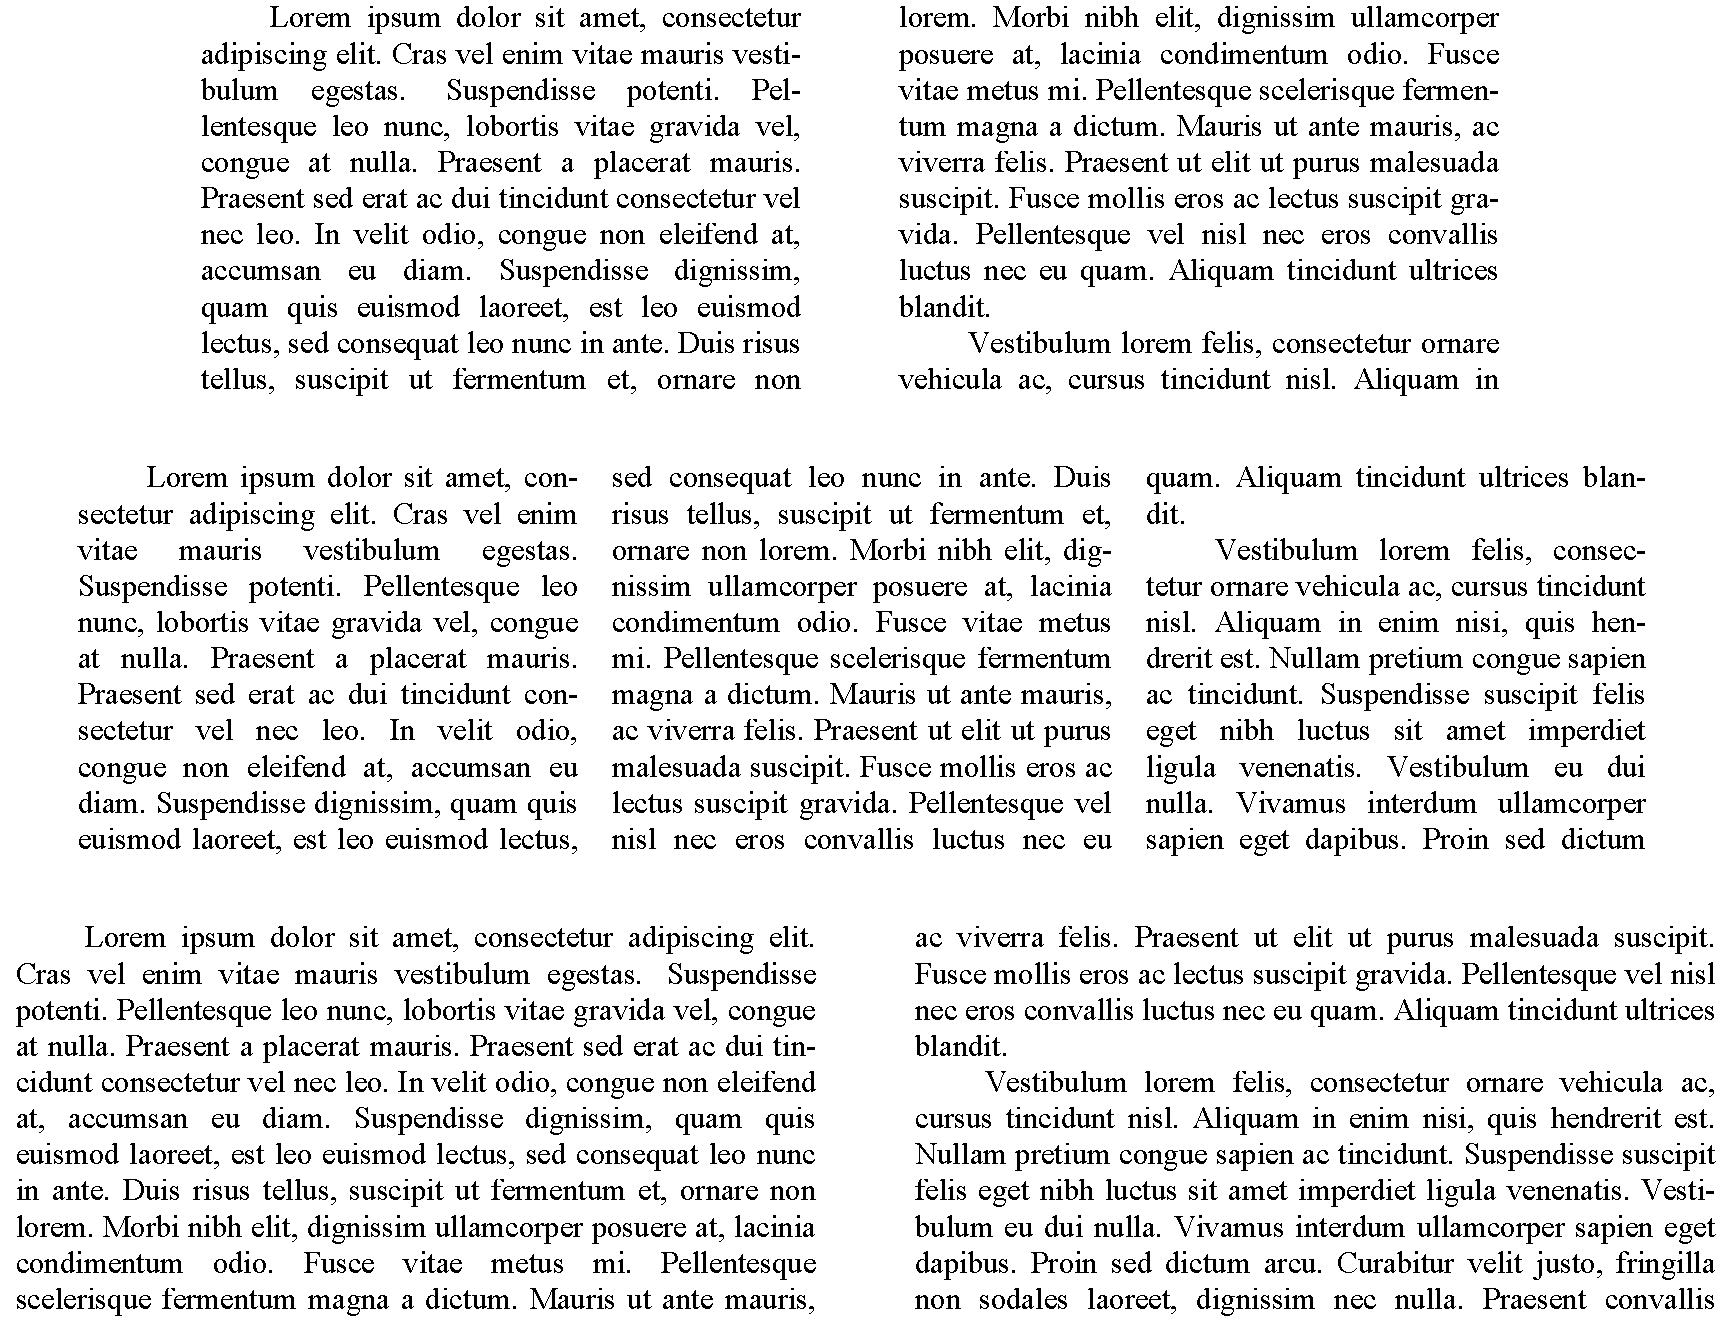
\includegraphics[width=\textwidth]{gfx/renderings}
 \caption[Sample renderings from the Acrobat plugin]{Sample renderings from the Acrobat plugin at page widths of 42, 48, and 54~em. \textbf{NOTE TO SELF: ADD BOUNDING BOXES}}
 \label{fig:renderings}
\end{figure}

The decision to use Acrobat as an eBook `emulator' stemmed once again from the available existing COG-based tools (see section \ref{sec:srcdoc}, as well as the extensive API and developer support available for Acrobat.

Since, by the point the document is to be displayed in Acrobat, most of the computationally expensive typesetting has already been carried out, the algorithm used to lay out the lines of the galleys can be very simple. The plugin chooses the most appropriate galley width to lay out, based on the current page width, and according to some measure of aesthetics, and then simply lays the document out line by line, with appropriate vertical spacing, until no more lines will fit in the current column. Any subsequent columns which will fit on the same page are then laid out in the same manner.

For convenience of testing, the plugin also automatically resizes the page to that of the window of Acrobat, and re-lays out the text on the fly, allowing various combinations of page sizes, zoom levels, and aspect ratios to be trialled.
Some sample renderings from the Acrobat plugin are shown in Figure~\ref{fig:renderings}.

\section{Layout Considerations}
\begin{figure}
 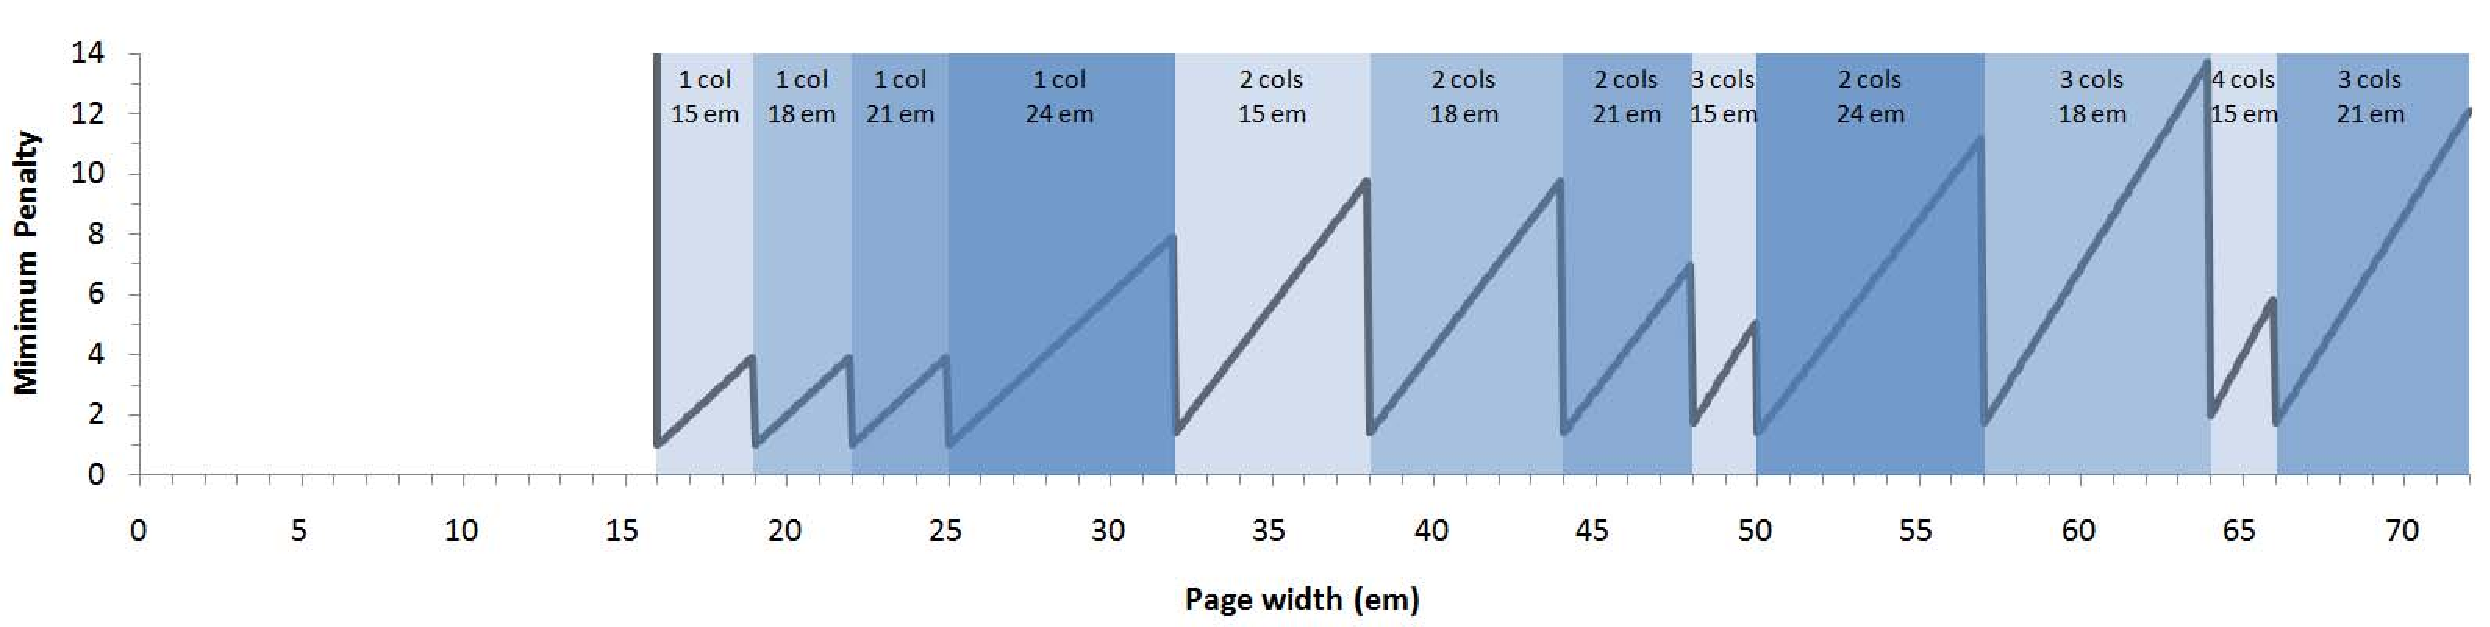
\includegraphics[width=\textwidth]{gfx/graph-em}
 \caption[Graph of minimum penalty values]{Graph showing the minimum penalty value of all galleys in a reflowable document, over a range of page widths. The particular document used contained four galleys; these were rendered at widths of 15, 18, 21 and 24~em, with a minimum gutter width of 1~em. Each vertical band highlights a range of page widths within which only the horizontal spacing of the page is altered. The boundaries between vertical bands represent a switch between galley renderings\ed{}the galley used and number of columns is as annotated on the graph.}
 \label{fig:penaltygraph}
\end{figure}
Since galleys of text lend themselves to being used in a columnar format, a method of fitting columns appropriately to the available page width must be devised. A sensible first approach is simply to calculate how many columns of each galley rendering will fit, by adding the galley width to a specified minimum inter-column spacing, and dividing the page width by this. The remainder of this division will then specify the total extra amount of horizontal whitespace required, which can then divided up and inserted between the columns. A simple measure of aesthetic quality here is to apply a linear penalty for any extra whitespace required, as we seek to keep page margins and column gutters to a minimum.

%\begin{math}
%N_\text{cols}=\left\lfloor\frac{W_\text{page}}{W_\text{galley}+W_\text{ICS}}\right\rfloor
%\end{math}

As the page width increases, so must the widths of the inter-column gutters. In accordance with the extra-whitespace penalty, each galley rendering will produce penalties which vary in a sawtooth manner as the width of the page is increased. With a careful choice of galley widths, when these sawtooth penalties are overlaid, and the galley producing the minimum penalty chosen at each page width, a flatter and finer-toothed penalty graph emerges, as shown in figure~\ref{fig:penaltygraph}.

In addition to penalising extra whitespace, wider columns should, in general, be favoured over narrower ones, i.e.~for a given page width, fewer, wider columns are generally considered preferable to a greater number of narrower columns. By multiplying the existing penalty by a smaller-than-linear function of the number of columns (experiments have been carried out with both logarithms and roots) the penalty may be subtly increased for greater numbers of columns. The formula for the penalty used in figure~\ref{fig:penaltygraph} is $P = (C + W_{ex})\cdot\sqrt{N_{cols}}$, where $P$ is the penalty, $W_{ex}$ is the extra whitespace required to be inserted, $N_{cols}$ is the number of columns which are required to fill the width of the page, and $C$ is a positive constant. The purpose of the constant is to prevent the penalty from ever evaluating to zero, which would have the effect of disregarding the weighting of the number of columns. Figure~\ref{fig:penaltygraph} uses $C=1$.
%eg what sort of layouts are we constricted to, and are they any good... cite Plass/Bringhurst

\section{Efficiency}
theoretically, how does it compare? Shove in lots of speculative Big Oh notation and try to sound authoritative. Or look at the algorithms used and
actually be authoritative :)



% \marginpar{Can we have one physical representation which fits to all devices \emph{and} is
% efficient? Should we perform some pre-processing to the document to tailor it to a particular
% device?}
% 
% Amazon's Kindle Store model provides a good example of the need for multipurpose documents\ed one
% purchase may be viewed on any number of platforms\ed the desktop app, the mobile phone app, the
% tablet app, and on the Kindle itself. Amazon does not currently provide any special dispensation for
% any of the platforms it supports\ed every one receives the same source document to display.
% Consequently, a Kindle book is effectively a jack of all trades, and master of none: instead of
% looking good on any one platform, the books look mediocre on \emph{every} platform. The real
% questions here are as follows:
% 
% \begin{itemize}
%  \item Is it possible to have one physical representation which typesets well on \emph{all}
% platforms whilst remaining efficient enough not to cause excessive battery drain?
%  \item Is it possible to identify invariant features common to many renderings to reduce the need
% for processing on the display device?
%  \item Should a more abstract, higher level of document be provided from which lower-level
% device-specific derivatives can be produced?
% \end{itemize}
%   
% The desire is to develop some document format which is neither as `solid' as a \pdf{} nor as
% `liquid' as \html{}, but somewhere in between (perhaps termed a \emph{malleable document}).
% Something which is mostly formed, but can be gently massaged to fit the display as necessary.
% 
% 
% \section{A Simple Implemenation}
% 
% 
% \marginpar{Mention paper here \cite{Pinkney2011}\ed appendix. Give brief overview of current
% system.}
% The majority of the work to date on this project is described in the paper \emph{Reflowable
% Documents Composed from Pre-rendered Atomic Components}\cite{Pinkney2011}, which was published and
% presented at the 2011 ACM Symposium on Document Engineering. It is also attached to this document as
% an appendix.
% 
% The paper outlines a very simple approach towards a malleable document format: the source document
% is simply rendered into `galleys' of text (see \cite{Pinkney2011}, section 3) multiple times, using
% a high-quality typesetting algorithm, with each rendering using a different galley width. The
% document is thus now displayable on multiple screen sizes (each width rendering may additionally be
% scaled by the display device to simulate point-size changes) without the need for the document to be
% expensively retypeset. The `best fit' rendering is chosen at display time, based on the available
% screen width and zoom level. The current implementation of this system is built around pre-existing
% tools for the \emph{ditroff} typesetting system\cite{Kernighan1982} and Component Object Graphic
% PDF\cite{Bagley2003}.
% 
% \subsection{Efficiency}
% \marginpar{Computational\cite{Knuth1981} \& space.}
% It is clear that computational efficiency must be maximised in order to minimise processor usage and
% battery drain. In order to do this, it will almost certainly be necessary to sacrifice storage
% efficiency; that is, filesizes are likely to be bigger. This is not necessarily a problem. Storage
% is cheap and plentiful; currently it is far more practical and cost effective to increase storage
% space than battery life. For this reason, we shall not concern ourselves too much with producing
% documents with small filesizes, and shall instead concentrate on pre-computing as much of the
% typesetting as possible, whilst retaining flexibility.
% 
% \subsection{Handling of edge cases}
% \label{edgecases}
% \marginpar{Corner cutting? Adjusting spacing\ldots word/letter spacing, glyph reshaping.
% \cite{Bringhurst2008}}
% The work described in \cite{Pinkney2011} and outlined above does not contain any special handling
% for edge cases, although this will not be difficult to implement. In particular, the system is
% currently restricted to displaying text only in the exact manner in which it was rendered. As an
% example, let us assume that a particular point size has been selected (i.e.\ the zoom level has been
% fixed); the best fit galley is then chosen for the page width. It may be the case that this
% particular galley rendering, at this zoom level, on a page of this width results in large margins.
% Perhaps the next galley size up is too wide to display. Currently, the penalty is simply to have to
% put up with these large margins. However, there are some simple tweaks which can be used to reduce
% how noticeable this effect is. As stated in section~\ref{goodtypesetting}, whilst performing
% justification, it is occasionally appropriate to adjust letter spacing and glyph widths, in addition
% to word spacing. Whilst readjusting these three
% parameters \emph{after} justification has taken place may reduce the typesetting quality (by making
% any of them larger or smaller than allowed by the justification rules) in certain cases it may be
% acceptable to do so, to fit the pre-rendered galley lines to a different width. Using the current
% implementation, it is particularly simple to adjust the word spacing\ed in the PDFs produced, each
% word is stored distinctly, and so can be repositioned as necessary. It is also very simple to
% reshape the glyphs, to either stretch or shrink them laterally. All PDF drawing operators are
% executed in accordance with the current \emph{transformation matrix}, which alters the coordinate
% system\cite{Adobe2001}. Glyph reshaping can thus easily be performed on any word or line by altering
% this before calling the requisite drawing operator. It is more difficult to alter the letter
% spacing, particularly in the current implementation, as this will involve looking up font metrics,
% and will be comparatively inefficient.
% 
% 
% \subsection{Examples of these principles in practice}
% Of particular interest and relevance to this thesis, is Amazon's recently announced Silk web browser
% for their new Kindle Fire platform. Silk uses a similar paradigm to that outlined in
% \cite{Pinkney2011} in order to serve web pages to the Kindle Fire, in a manner that requires less
% processing by the device itself. Amazon makes use of its extensive computing power in its Cloud
% service to prerender any webpage requested through Silk. The output is tailored specifically to the
% device, enabling, for instance, layout of tables, or image scaling, to be performed on the Cloud
% servers rather than locally on the device. Amazon has produced a five minute technical overview
% video, available at \verb+http://www.youtube.com/watch?v=_u7F_56WhHk+
% 
% 
% \subsection{Anticipated extensions}
% \marginpar{Newspaper galley creation guidelines? look into\ldots}
% Since the current work relies heavily on the setting of text into galleys, it would probably be
% pertinent to research newspaper galley creation guidelines. These may be difficult to come by, since
% newspapers have been electronically typeset for much of the last three decades. Nevertheless, the
% information must be available somewhere, and could prove invaluable.
% 
% \marginpar{Device profiles\ldots what is appropriate? Image resolution? Page width renderings for
% specific screen size?}
% At some point, it will probably prove necessary to tailor the output document to the specific device
% for which it is intended. Accordingly, profiles for these devices must be devised, which contain all
% the necessary attributes to produce a document to fit. For example, image resolution must be
% considered. Is there a necessity to use hi-resolution images for a document which is to be displayed
% on a mobile phone screen? Perhaps not. Whilst a large image may be scaled down to fit, unless the
% image is required to be zoomable, it seems sensible to precompute this scaling, and remove the need
% for the device to perform it each time the image is displayed. Similarly, it may be sensible to
% generate galleys only in sizes appropriate to the device. A mobile phone is clearly going to require
% narrower renderings than a tablet, for example. Whilst each document \emph{could} include many
% resolutions of each image, and a vast range of galley width renderings suitable for many devices, it
% seems rather wasteful to do so when
% these tailored versions can easily be produced. It is envisaged that such a system would run on a
% user's desktop or laptop PC, which would store the canonical, high-level representation of the
% document, and that the apparent copying of that document to a display device would in fact create a
% bespoke version of the document, specifically to fit the device, yet still with enough flexibility
% to allow the font size to be changed within sensible limits.
% 
% \marginpar{Perhaps suggest using vector images where possible?}
% 
% 
% \subsection{Conclusions}
% \marginpar{Need to balance time/complexity against appearance. Comparable to eg Plass/Knuth? thus
% need some way to quantify appearance\ed some form of metrics needed for this. Needs
% investigation\ldots}
% Computational efficiency is easily quantifiable, both on a theoretical level, and experimentally.
% Typesetting quality, however, is harder to quantify. In order to show whether this system can
% produce consistently better results than a standard \ebook{} layout engine, some method must be
% derived in order to compare them. This may be based on a point-scoring system, in a similar manner
% to \TeX{}\cite{Knuth1984}, or perhaps by more qualitative means, such as human judgement. In either
% case, both these factors must be balanced against one another, striving to reduce computational
% efficiency whilst maintaining typesetting quality.
% 
% 
% 
% 
% 
% \section{Introduction}
% In recent years, the consumption of documents on mobile devices, such as eBook readers, has
% increased dramatically. However, the visual quality of a document on these devices is often lacking,
% when compared to other digital document systems (see figure \ref{kindle}). The result of an eBook
% reader's layout engine is often visually unappealing, with uneven spacing in consecutive lines of
% text, poor justification, and the lack of a sophisticated hyphenation system.
% 
% This is a far cry from the quality of typesetting available from PDF or PostScript documents. These
% vector-based, de\-vice-in\-de\-pen\-d\-ent page description languages are able to create a digital
% version of the document that is identical to its printed counterpart. These page description
% languages, coupled with high-quality typesetting systems (such as \TeX{}, troff or Adobe InDesign)
% have produced an expectation that digital documents will be of similar quality to that achievable
% through hand composition. \TeX{} and Adobe InDesign, in particular, have excellent support for many
% of the subtle nuances used by hand compositors, which are often overlooked by more basic typesetting
% packages (e.g.~automated support for kerning and ligatures). This quality does not come without a
% price: the algorithms used to calculate the layout are computationally expensive and so are run only
% once, to produce a PDF with a fixed layout targeted at a fixed page size.
% 
% eBook readers, it seems, have had to take a step backwards to simpler (and, therefore, less
% computationally expensive) algorithms to maximise the battery life of the device. The result is that
% the high-end hyphenation, kerning, and ligature support has had to be sacrificed and the on-screen
% result is reminiscent of the output of an HTML rendering engine or a very basic word processor.
% 
% This paper investigates an alternative approach to generating the display for an eBook reader. Here,
% the text is pre-rendered (using a high-quality typesetting algorithm) in several column widths,
% prior to display, when the document is created. At view time, the most appropriate column width is
% selected for display, the system balancing between excessive white space and multiple columns.
% Section~\ref{problems} examines the problems posed by current eBook readers in further detail, while
% section~\ref{solution} presents our initial prototype solution to some of these problems.
% 
% \section{Problems with Current eBook Readers}
% \label{problems}
% Three formats currently dominate the eBook market: EPUB and Mobipocket, which allow the document to
% be formatted to fit the device, and PDF, which does not. (Amazon's proprietary Kindle format is
% derived from Mobipocket; PDF and EPUB are open standards.) Both the EPUB and Mobipocket formats are
% largely based on XHTML. Whilst the use of XML-derived formats allow the semantic structure of
% documents to be very well defined, in general their presentation can only be specified in a very
% loose manner. The user is often presented with a choice of typefaces and point sizes, allowing the
% reader software to render the document in essentially any arbitrary way it chooses.
% 
% Conversely, PDF is entirely presentation-oriented, stemming from its origin of being compiled
% PostScript. PDF, therefore, will often include no information on the semantic structure of the
% document, and will consist simply of drawing operators which describe the document pages. There is
% no compulsion for these drawing operators to render the page in an order that might be considered
% sensible: for example, if a PDF generator program decided to render every character on a page in
% alphabetical order, or radially outwards from the centre, the resulting file would still be
% semantically valid, and the result might well be unnoticeable to the end user. This lack of imposed
% semantic structure can make it difficult to infer the best way to `unpick' PDF files to allow their
% content to be reflowed into a new layout.
% 
% Since an XHTML-derived format has no fixed presentation associated with it, this must be calculated
% each time the document is displayed, in a similar manner to the way an interpreted programming
% language needs to be interpreted each time it runs. For an eBook reader to maximise its battery life
% (the human reader will be annoyed if the device dies just before the climax of a novel!), the
% `interpretation' needs to be as simple as possible\,---\,i.e.~the algorithm used must not be too
% complex, since the more CPU cycles spent executing it, the less time the CPU can spend idle, and
% hence the greater the drain on the battery. Furthermore, the longer that is spent formatting the
% output, the longer the delay between page turns on the device, and with the speed of CPUs used in
% these devices (<~500~MHz) it does not take too large an increase in computation for the page turn to
% become noticeable.
% 
% \begin{figure}
%     \centering
%     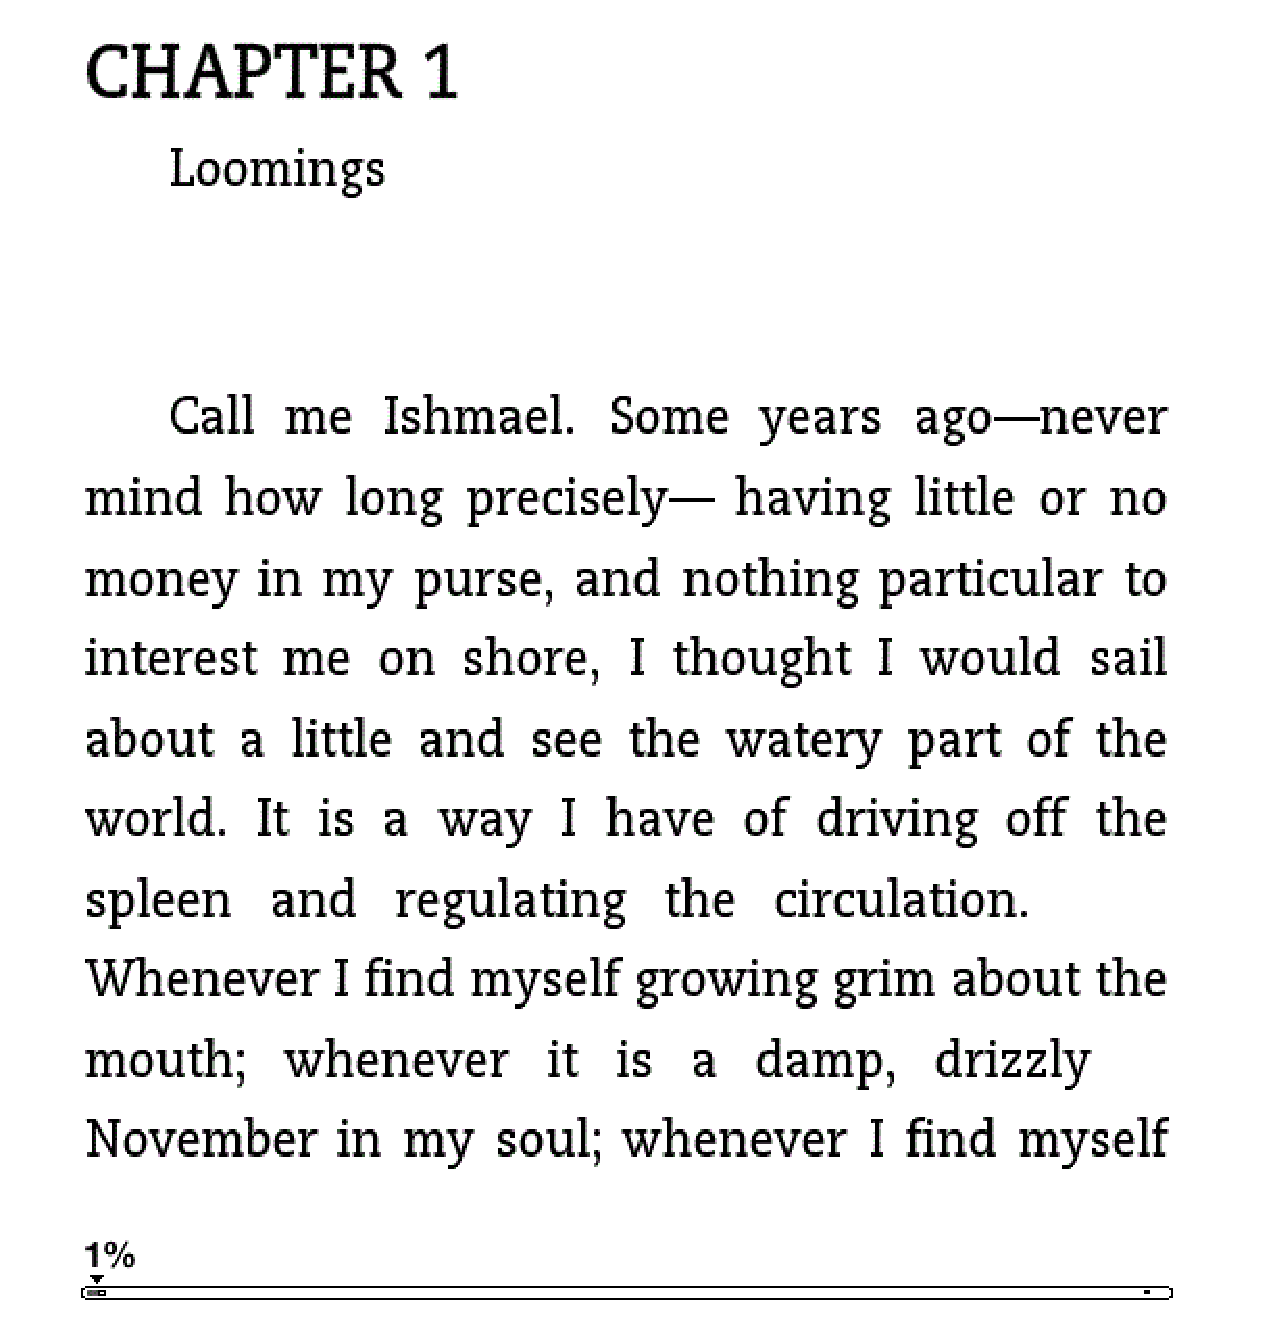
\includegraphics[width=\textwidth]{gfx/screen_shot-42583}
%     \caption[An example of typesetting on the Kindle]{The Kindle 3 appears to primarily use
% justified text, falling back to ragged-right when
% inter-word spacing would become too large.}
%     \label{kindle}
% \end{figure}
% 
% \subsection{Hyphenation and Line-Breaking}
% eBook readers typically use a `greedy' algorithm to lay out their text\,---\,that is, they place as
% many words as will fit onto the current line without exceeding it, then start a new line and
% continue. Although this algorithm is optimal in that it will always fit text onto the fewest
% possible lines, it often causes consecutive lines to have wildly varying lengths, accentuating
% either the `ragged-right' effect of the text, or, in the case of justified text, the inter-word
% spacing. In general, eBook readers will only hyphenate in extreme cases\,---\,indeed the Kindle~3
% seems not to do so at all. Knuth and Plass\cite{Knuth1981} developed a more advanced line-breaking
% algorithm (now used by \TeX{}) which attempts to minimise large discrepancies between consecutive
% lines by considering each paragraph as a whole. \TeX{} also uses the hyphenation algorithm designed
% by Liang\cite{Liang1983}, which has been ported to many other applications.
% 
% \subsection{Other Typographical Techniques}
% Other techniques employed during hand-type\-set\-t\-ing and high-qua\-l\-ity electronic typesetting
% include the use of kerning and of ligatures. Kerning involves altering the spacing between certain
% glyph pairs in order to produce more consistent letter spacing, whilst ligatures are sin\-gle-glyph
% replacements for two or more single glyphs which may otherwise have clashing components. Some
% examples of these are shown in figure~\ref{kern-lig}.
% Kerning requires a table of kern-pairs, specific to each font; values from this table must then be
% looked up for every pair of adjacent glyphs in the document. Ligatures may or may not need to be
% inserted: if the component characters of the ligature lie over a potential hyphenation point, it
% cannot be decided whether to replace them with the ligature until it is known whether the
% hyphenation point needs to be used.
% 
% 
% \begin{figure}
% 
%     %\centering
%     \vspace{-24pt}
%     {\Huge \textbf{
%     \begin{tabbing}
%     \hspace{0.1in} \= T\mbox{}o \= A\mbox{}V \= V\mbox{}. \= W\mbox{}a\hspace{0.3in}\= f\mbox{}i \=
% f\mbox{}l\\
%     \> To \> AV \> V. \> Wa \> fi \> fl
%     \end{tabbing}
%     }}
%     \caption[Examples of kerning and ligatures]{Examples of various letter-pairs and their kerned
% (left) or ligature (right)
% equivalents, as typeset by \TeX{}.}\vspace{-3pt}
%     \label{kern-lig}
% \end{figure}
% 
% 
% % % % % % % % % % % % % % % % % % % % % % % % % % % % % % % % % % % % % % % % % % % % % % % % % % %
% 
% 
% \section{A Galley-Based Approach}
% \label{solution}
% %note that storage is \textbf{not} at a premium, but battery life/processor are.
% %Prerender as much as possible, ie at compile-time
% %Layout then becomes simple. Allows arbitrarily complex layout with no overheads at runtime
% %Include a tree so the semantic structure of the document is explicit
% Our proposed solution, of precomputing several text variants, revisits an approach to typesetting
% from before the advent of desktop publishing. In the days before DTP, newspaper articles were
% typeset into long columns known as \emph{galleys}. Since all columns in the newspaper would be of
% uniform width, all articles could be typeset into galleys of the same measure, and then broken as
% necessary between lines, in order to slot into the final layout of the newspaper. Once the text has
% been set in this manner, with appropriate hyphenation and justification, the individual lines can be
% treated as atomic units that will never have to be re-typeset. In essence, each article is
% `compiled' only once, but can be used anywhere in the final layout without penalty.
% 
% %could this all be one paragraph?
% 
% It is this behaviour we wish to emulate. So long as the atomic components of the document are
% tightly specified, and the reader software can obey the associated drawing instructions (essentially
% treating them as pre-typeset blocks), the resulting display of the document will be of as high
% typographic quality as that of the original galley, and the requirement for further computation will
% be vastly reduced. In order to permit aesthetic layout for a wider range of screen sizes, it seems
% sensible to create a document containing multiple renderings of the same content, and simply
% choosing the `best fit' rendering when the document is displayed.
% 
% %Something about ideal text measure\cite{Bringhurst2008}
% 
% %need to say several renderings included
% 
% 
% \subsection{A Sample Implementation}
% Our sample implementation is built around our existing work in PDF and Component-Object Graphics
% (COGs)\cite{Bagley2003}, but there is no reason why it could not be implemented in any other format
% capable of tightly specifying page imaging operations. It builds on existing software, principally
% \emph{pdfdit}, in conjunction with \emph{COG Manipulator}, as these tools are already capable of
% producing modular documents with tightly specified rendering.
% 
% 
% \subsubsection{The COG Model}
% %summary of cogs, what I've changed, ie line-level rather than default paragraph level. Put in tree
% to retain par details
% The Component Object Graphic (COG) model was developed to enable the reuse of semantic components
% within PDF documents, by breaking the traditional graphically-monolithic PDF page into a series of
% distinct, encapsulated graphical blocks, termed COGs. In its original incarnation, the COG model did
% not account for any relationship between individual COGs\,---\,it was simply designed as a method by
% which document components could be easily reused or reordered. The COGs it generates are largely at
% the granularity of a paragraph, and can still be imaged onto the page in any arbitrary order,
% independent of reading order.
% 
% In order to implement our galley-based design, it is necessary to decrease this granularity, such
% that each line of text is represented by a separate COG. However, it is also important that the
% semantic structure of the document is explicitly stored. This is principally so that the reading
% order of the COGs is maintained, and also so that the reader software can identify paragraphs,
% headings etc.~to enable them to be laid out correctly.
% 
% The COG model takes advantage of the fact that the PDF specification allows the content of a page to
% be described by an array of streams of imaging operators, rather than the more commonly encountered
% single, monolithic stream. Unfortunately, this array can only be one-di\-men\-sional, meaning that
% while it can enforce the reading order, it cannot be used to, say, group lines into paragraphs.
% Since the PDF specification allows essentially arbitrary insertion of data structures into a
% document (PDF readers which do not recognise these will simply ignore them), this flexibility was
% used to embed a simple tree structure representing the paragraphs, in parallel to the COGs
% themselves (an example of which is shown in figure~\ref{tree}). At the level of its leaves, this
% tree simply contains pointers to the COGs which make up the content of the document. In the simplest
% case, where the document contains only one rendering (and thus the pa\-ra\-graph-level items have
% only one child) the COGs pointed at by the leaves can simply be rendered in order, adding vertical
% space as appropriate.
% 
% 
% \begin{figure}
%     \centering
%     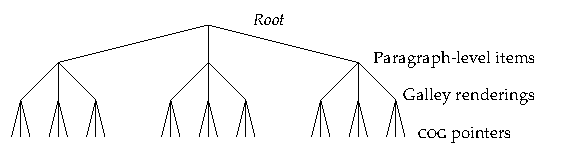
\includegraphics[width=\textwidth]{gfx/tree}
%     \caption[A simple document structure tree]{A simple document structure tree. The first level
% below the root represents all
% paragraph-level items: headings, paragraphs, figures etc. These items have one child for each galley
% rendering of the document. These in turn have one child for each COG comprising their
% content\,---\,in the case of a paragraph or heading: its lines; in the case of a figure: the figure
% itself and any associated caption.}\vspace{-3pt}
%     \label{tree}
% \end{figure}
% 
% \subsubsection{The Source Document}
% Since the majority of available tools for producing COGged PDFs rely on the typesetting package
% \emph{ditroff}, it was decided to use this as the basis for the source document. Ditroff is
% particularly amenable to many of the features required here\,---\,it is quite happy to have its page
% length set to large numbers\,---\,one sample document used a page length of 2000 inches
% (approximately 50 metres) with no complaints from ditroff. The line length was set to a small value
% (approximately two inches) in order to produce a narrow column of text. Following this, the actual
% document content was inserted several times, and the line length incremented, producing one document
% effectively containing multiple galley renderings of the same content.
% 
% 
% %- troff source doc, long page, narrow column, creating galley
% 
% \subsubsection{pdfdit}
% Having generated the source document, it was processed with ditroff to generate the intermediate
% code used to feed each typesetter post-pro\-cessor. This output is very expressive, and, unlike
% \TeX's DVI, contains enough information that post-processors are easily able to locate the start and
% end of lines and paragraphs within the document. This meant that only minimal changes were needed to
% be made to the \emph{pdfdit} package described in \cite{Bagley2003} to implement our design.
% 
% The first change necessary was to decrease the granularity of the output COGs, producing them at the
% line level, rather than at the paragraph level. Secondly, some method of generating the requisite
% tree representing the document structure was required. This was solved by simply using the point at
% which the original version of pdfdit would have started a new paragraph-level COG, and, instead,
% starting a new paragraph-level block entry in the document structure tree. Each subsequent
% line-level COG produced can then be added as a child of this block.
% 
% Once the entire output file has been parsed, the tree representations o-f the various width galleys
% are amalgamated per-paragraph, as indicated in figure~\ref{tree}, and finally the PDF file is
% serialised, replete with COGs and content tree.
% 
% 
% %Note also the inclusion of baseline/indent?
% 
% %summary, plus what's changed (similar to the above)
% 
% 
% 
% \subsubsection{Acrobat Plugin}
% \begin{figure}
%  \centering
%  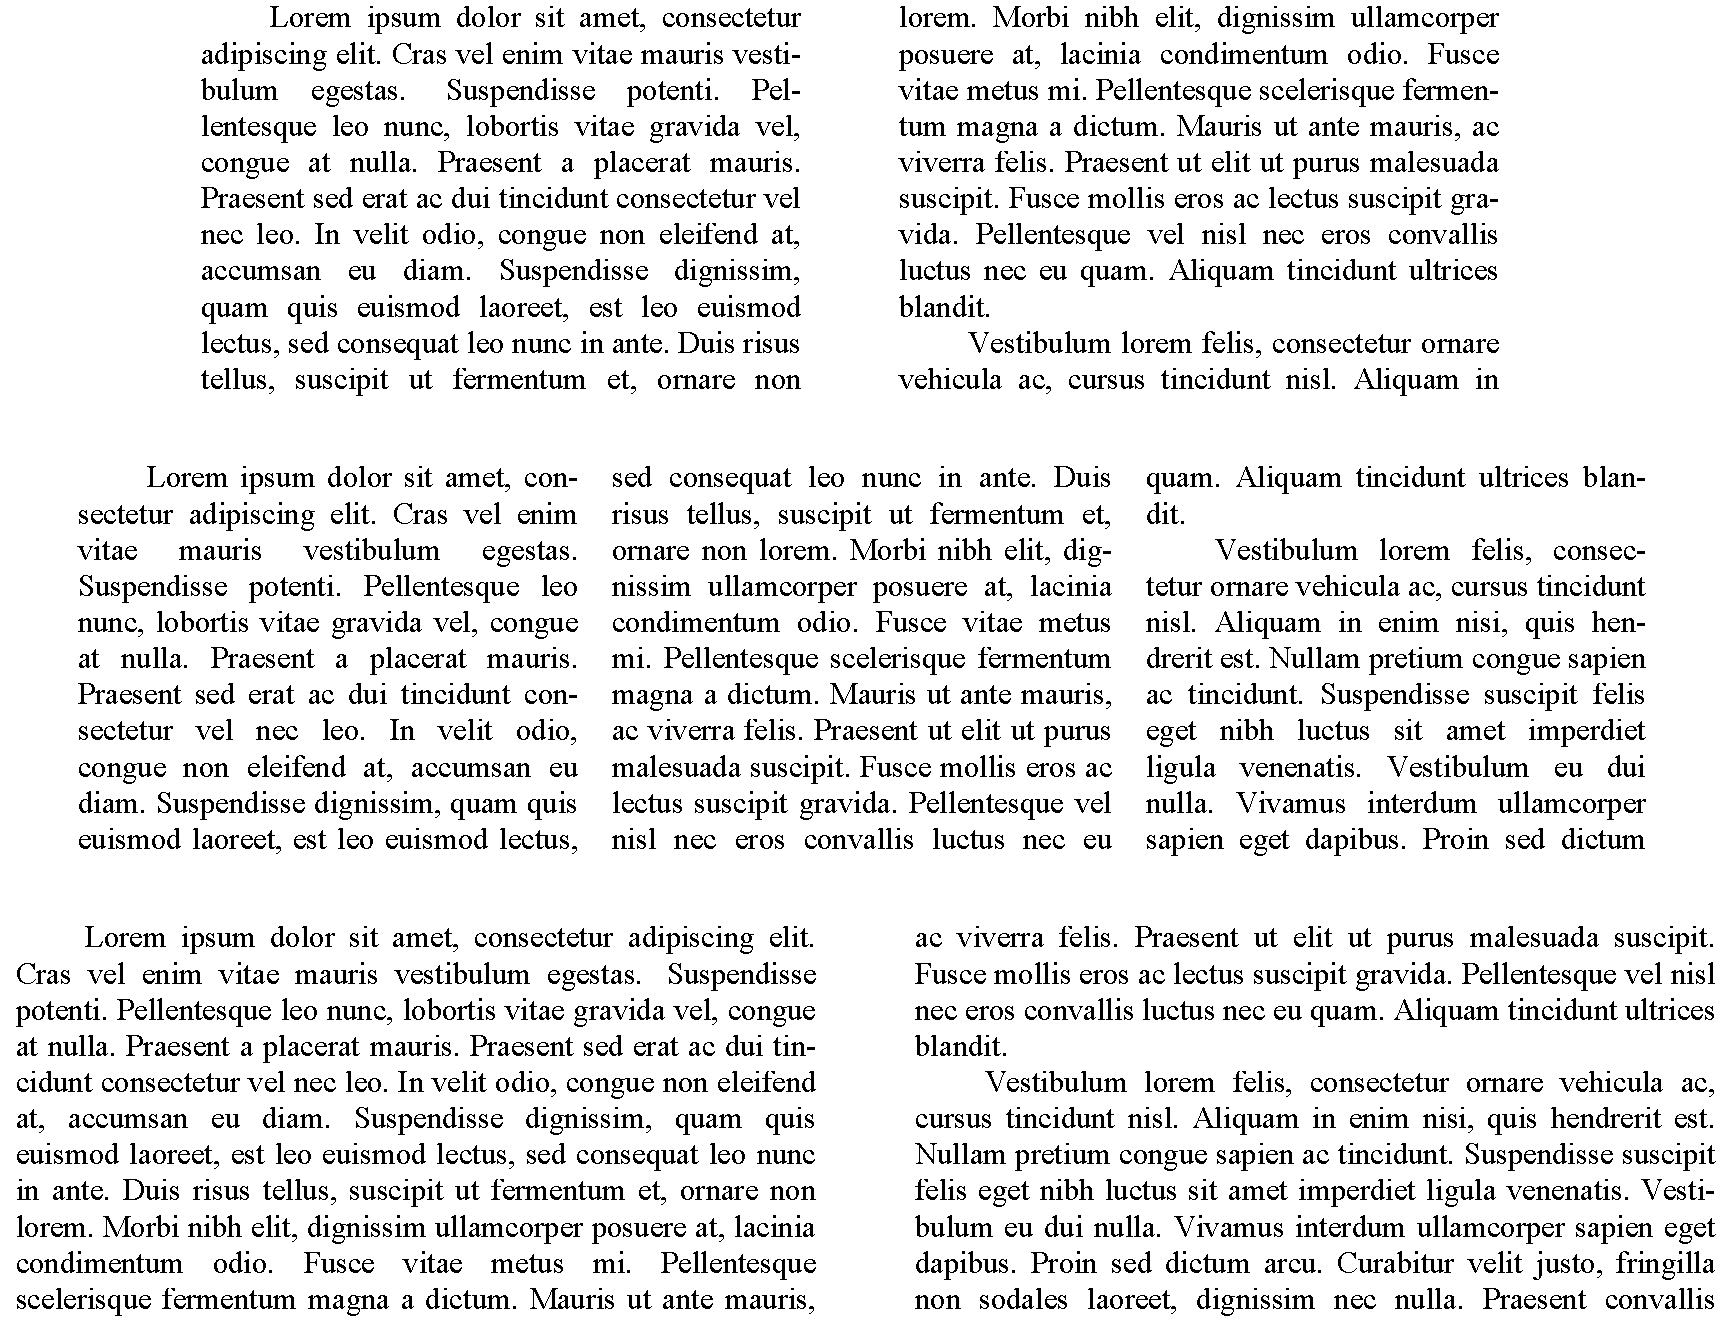
\includegraphics[width=\textwidth]{gfx/renderings}
%  \caption[Sample renderings from the Acrobat plugin]{Sample renderings from the Acrobat plugin at
% page widths of 42, 48, and
% 54~em.}
% \end{figure}
% 
% \begin{figure}
%     \centering
%     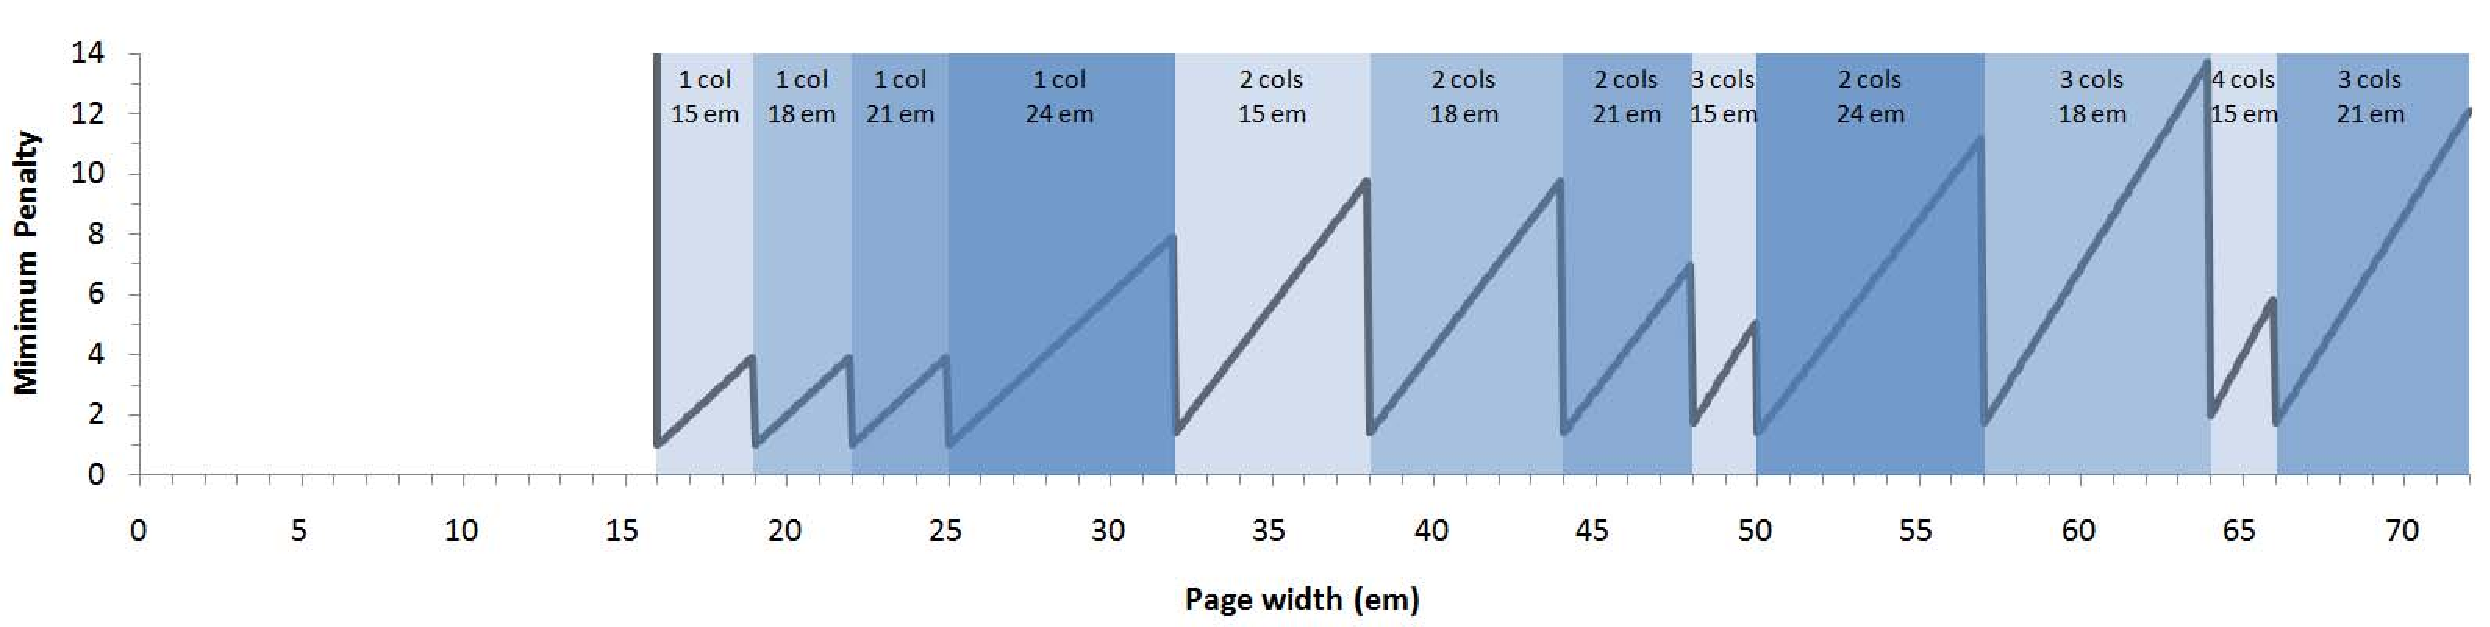
\includegraphics[width=\textwidth]{gfx/graph-em}
%     \caption[Layout Penalty Graph]{Graph showing the minimum penalty value of
% all galleys in a reflowable document, over a
% range of page widths. The particular document used contained four galleys; these were rendered at
% widths of 15, 18, 21 and 24~em, with a minimum gutter width of 1~em. Each vertical band highlights a
% range of page widths within which only the horizontal spacing of the page is altered. The boundaries
% between vertical bands represent a switch between galley renderings\,---\,the galley used and number
% of columns is as annotated on the graph.}\vspace{-3pt}
%     \label{graph}
% \end{figure}
% 
% The decision to use Acrobat as an eBook `emulator' stemmed once again from the available existing
% COG-based tools, as well as the extensive API and developer support available for Acrobat. Moving a
% COG on a PDF page is as simple as deleting its associated spacer object from the content array of
% the page, creating a new spacer containing the COG's desired new position, and then adding that back
% to the content array.
% 
% Since, by this point, most of the computationally expensive typesetting has already been carried
% out, the algorithm used to lay out the lines of the galleys can be very simple. The plugin chooses
% the most appropriate galley width to lay out, based on the current page width, and according to some
% measure of aesthetics, and then simply lays the document out line by line, with appropriate vertical
% spacing, until no more lines will fit in the current column. Any subsequent columns which will fit
% on the same page are then laid out in the same manner.
% 
% %Probably don't need this:
% %For convenience of testing, the plugin also automatically resizes the page to that of the window of
% %Acrobat, and re-lays out the text on the fly, allowing various combinations of page sizes, zoom
% %levels, and aspect ratios to be trialled.
% 
% \subsubsection{Layout and Metrics}
% 
% 
% Since galleys of text lend themselves to being used in a columnar format, a method of fitting
% columns appropriately to the available page width must be devised. A sensible first approach is
% simply to calculate how many columns of each galley rendering will fit, by adding the galley width
% to a specified minimum inter-column spacing, and dividing the page width by this. The remainder of
% this division will then specify the total extra amount of horizontal whitespace required, which can
% then divided up and inserted between the columns. A simple measure of aesthetic quality here is to
% apply a linear penalty for any extra whitespace required, as we seek to keep page margins and column
% gutters to a minimum.
% %\begin{math}
% %N_\text{cols}=\left\lfloor\frac{W_\text{page}}{W_\text{galley}+W_\text{ICS}}\right\rfloor
% %\end{math}
% 
% As the page width increases, so must the widths of the inter-column gutters. In accordance with the
% extra-whitespace penalty, each galley rendering will produce penalties which vary in a sawtooth
% manner as the width of the page is increased. With a careful choice of galley widths, when these
% sawtooth penalties are overlaid, and the galley producing the minimum penalty chosen at each page
% width, a flatter and finer-toothed penalty graph emerges, as shown in figure~\ref{graph}.
% 
% In addition to penalising extra whitespace, wider columns should, in general, be favoured over
% narrower ones, i.e.~for a given page width, fewer, wider columns are generally considered preferable
% to a greater number of narrower columns. By multiplying the existing penalty by a
% smaller-than-linear function of the number of columns (experiments have been carried out with both
% logarithms and roots) the penalty may be subtly increased for greater numbers of columns. The
% formula for the penalty used in figure~\ref{graph} is $P = (C + W_{ex})\cdot\sqrt{N_{cols}}$, where
% $P$ is the penalty, $W_{ex}$ is the extra whitespace required to be inserted, $N_{cols}$ is the
% number of columns which are required to fill the width of the page, and $C$ is a positive constant.
% The purpose of the constant is to prevent the penalty from ever evaluating to zero, which would have
% the effect of disregarding the weighting of the number of columns. Figure~\ref{graph} uses $C=1$.
% 
% %\vspace{-8pt}
% 
% \section{Conclusions and Future Work}
% This paper outlines our initial exploration of the idea of using pre-rendered galleys for eBooks. So
% far,  our initial implementation has generated multicolumn layouts that look acceptable, and we
% believe there is mileage in continuing to investigate this method. However, there is still a lot of
% work to be done. Firstly, a very simple formula is used to determine which column width variant to
% select, and we are investigating the suitability of other methods of determining aesthetically
% pleasing layouts (such as those outlined in
% \cite{Balinsky2009,Bringhurst2008,Goldenberg2002,Harrington2004,Johari1996,Purvis2003}). Also, our
% system does not currently allow the font size to be changed (since it is fixed when the galleys are
% created). One approach to allow the font size to be changed would be to scale smaller column width
% variants up to larger columns. For example, if the 15~em wide variant is scaled up to 18~em, then
% text would be scaled up by 20\%\,---\,the equivalent of converting 10~pt text to 12~pt.
% 
% It should also be noted that optimal placement of floating blocks cannot be `compiled out' in the
% same manner that hyphenation and line breaking can; these will still need to be positioned into the
% relevant places as the document is displayed. If the simple approach is taken that floats should be
% placed at the top of a column or after another float, a document layout somewhat reminiscent of this
% one will emerge, although the floats will inevitably tend to drift towards the end of the document,
% away from their desired position.
% 
% Finally, to confirm that this method has validity it needs to be implemented in an actual eBook
% system, rather than simulated in Acrobat. There, it will be possible to compare the performance of
% our system with both a normal eBook renderer, and one that has been enhanced to use a sophisticated
% hyphenation and justification algorithm.
% 
% %port to actual ebook platform. Try to get \TeX's line breaking algorithm going with it. optimise
% %rendered widths to get best coverage
% 
% %Note that figure placement may still be a problem - optimal positioning will probably involve some
% %lookahead. See Plass's thesis\cite{Plass1981}.
% 
% %The COG-like objects can actually be structured in a tree in non-pdf formats, so we don't need the
% %parallel tree.
% 
% %note that this relies on the lines being rendered *precisely* as specified, otherwise we'll only
% %end up with shoddy spacing again. Need to find a method by which ebook readers can do this, in a
% %similar manner to formxobjects in pdf
% 
% %include plaintext for emergencies? Cite Steve's paper??
% %Maybe allow new renderings to be saved within the document for later use?
% 
